\chapter{TEST \& DESIGN}\label{cha:test}
In this chapter the methods used for testing the mobile devices for different characteristics is described. 

\section{Accelerometer \& Gyroscope}\label{sec:test:motion}
I decided to collect the data via a web-page since JavaScript can access gyroscope and accelerometer data without any permission or knowledge from the user \cite[]{sensor:DeviceOrientation:spec}. This only require that the device has Internet and a browser installed, no additional installations and completely cross-platform. \\


For the measurements of the accelerometer a event listener is added:
\lstinputlisting{code/acc-listener.js}
In JavaScript there are two types of acceleration with and without gravity, which according to Mozilla means that \texttt{accelerationIncludingGravity} is acceleration made by the device. In context to \texttt{acceleration} not depending on influence of gravity only by the acceleration made on the device. But as I see it that acceleration is made because of gravity so it is just different point of views. Since iOS has the z-axes pointed at the opposite direction that gives an additional security bit, that's why that one is used in this test. The accelerometer also comes with the nice feature of \texttt{rotationRate} which is the acceleration made from the axes in alpha, beta and gamma direction, see~\Figureref{fig:device-axes}. \cite[]{sensor:accIncludingGravity} \\
\\
For the measurements of the gyroscope another event listener is added:
\lstinputlisting{code/gyro-listener.js}
The \texttt{DeviceOrientation} is using the same axes as the accelerometer but the gyroscope is measuring how much the device is rotating along the \texttt{alpha, beta} and \texttt{gamma} axes in degrees (\Figureref{fig:device-axes}). The \texttt{alpha} is between 0 and 360 degrees, \texttt{beta} -180 to 180 degrees and \texttt{gamma} -90 to 90 degrees. \citet{sensor:DeviceOrientation:spec}.

\subsection{Accelerometer \& Gyroscope-test I}
The recording of the first accelerometer test is done by taking thousand accelerator-data samples during a few seconds and saved in a CSV for analyzing.
\begin{figure}[H]
  \hspace{-2cm}
  \centering
  \begin{minipage}[c]{.23\textwidth}
    \centering
    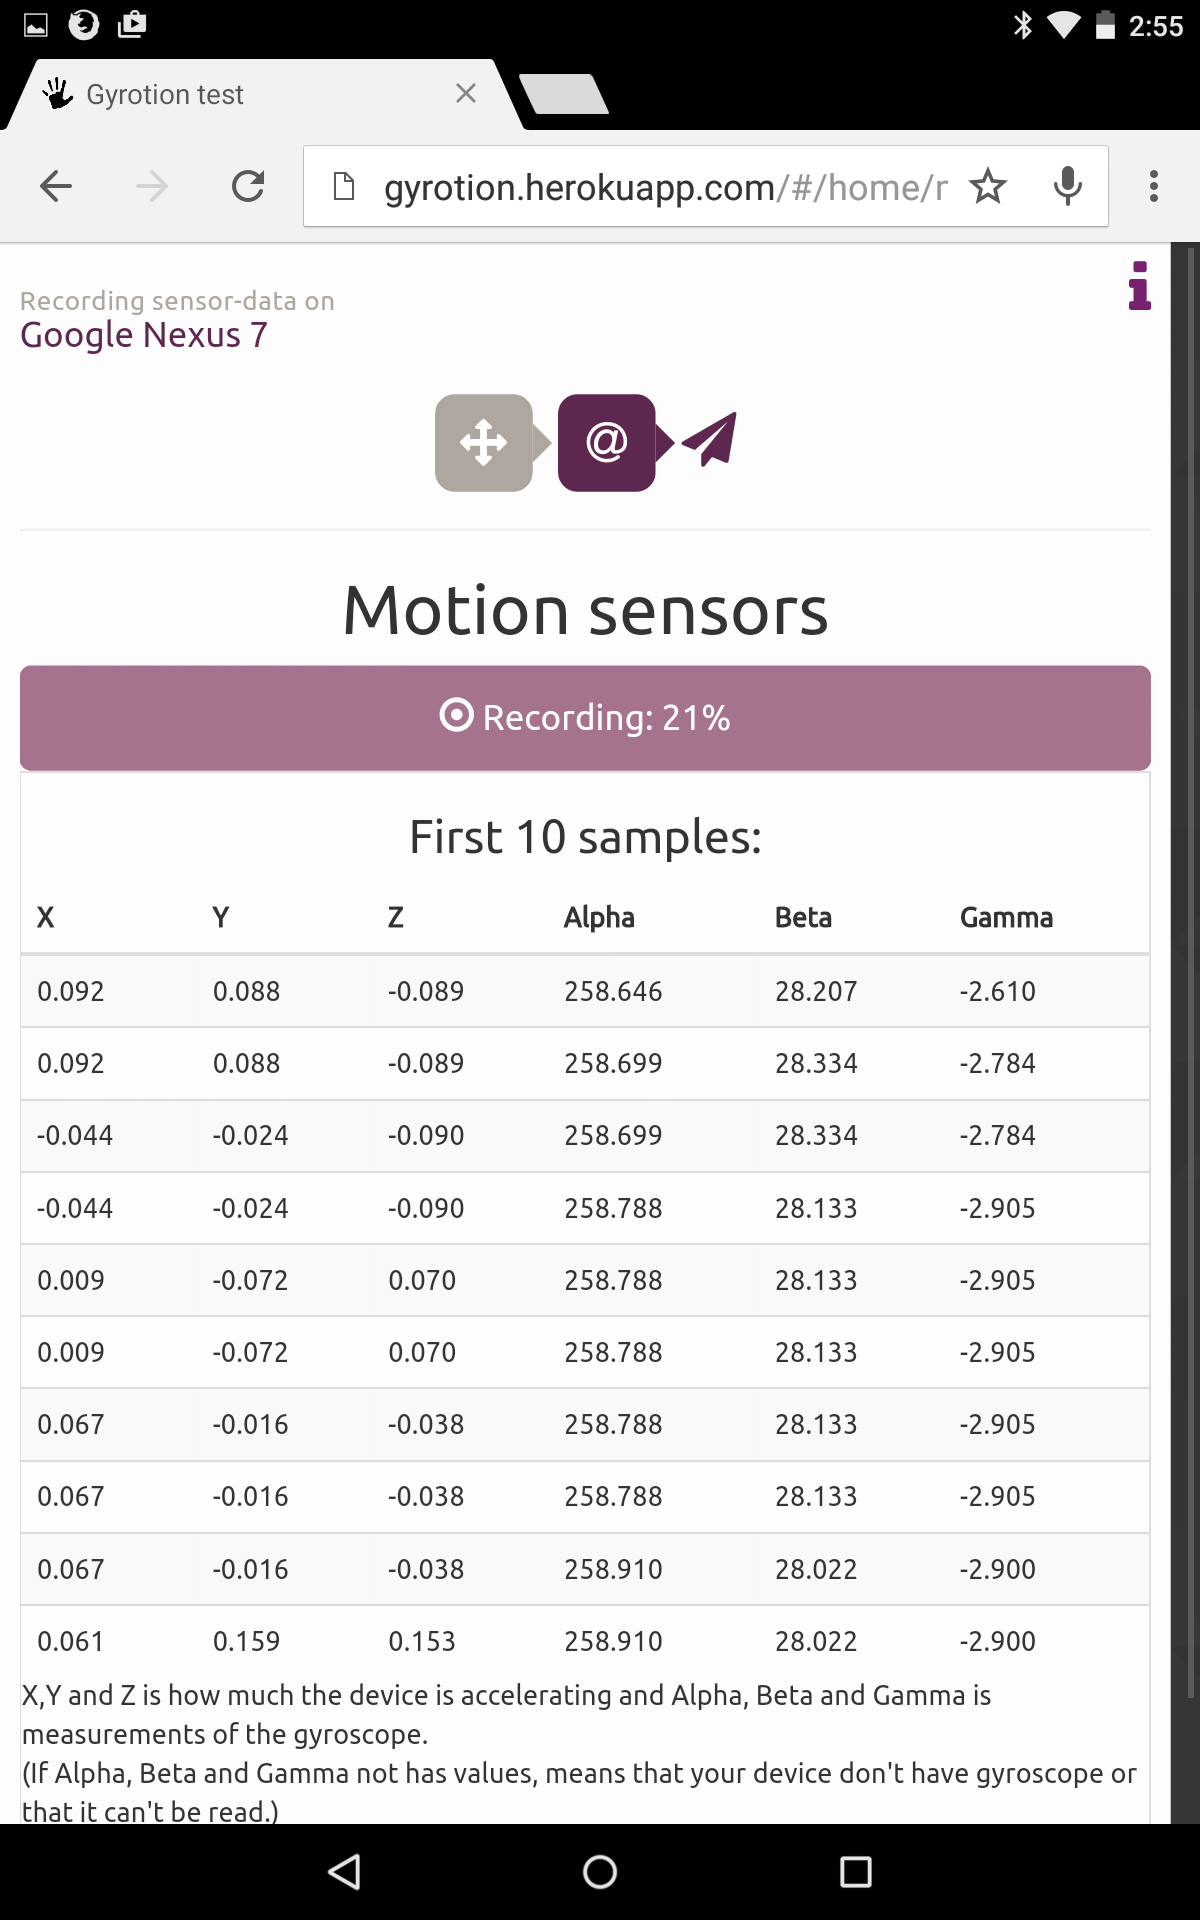
\includegraphics[scale=0.1]{img/Nexus-rec}
  \end{minipage}
  \hspace{2cm}
  \begin{minipage}[c]{.23\textwidth}
    \centering
    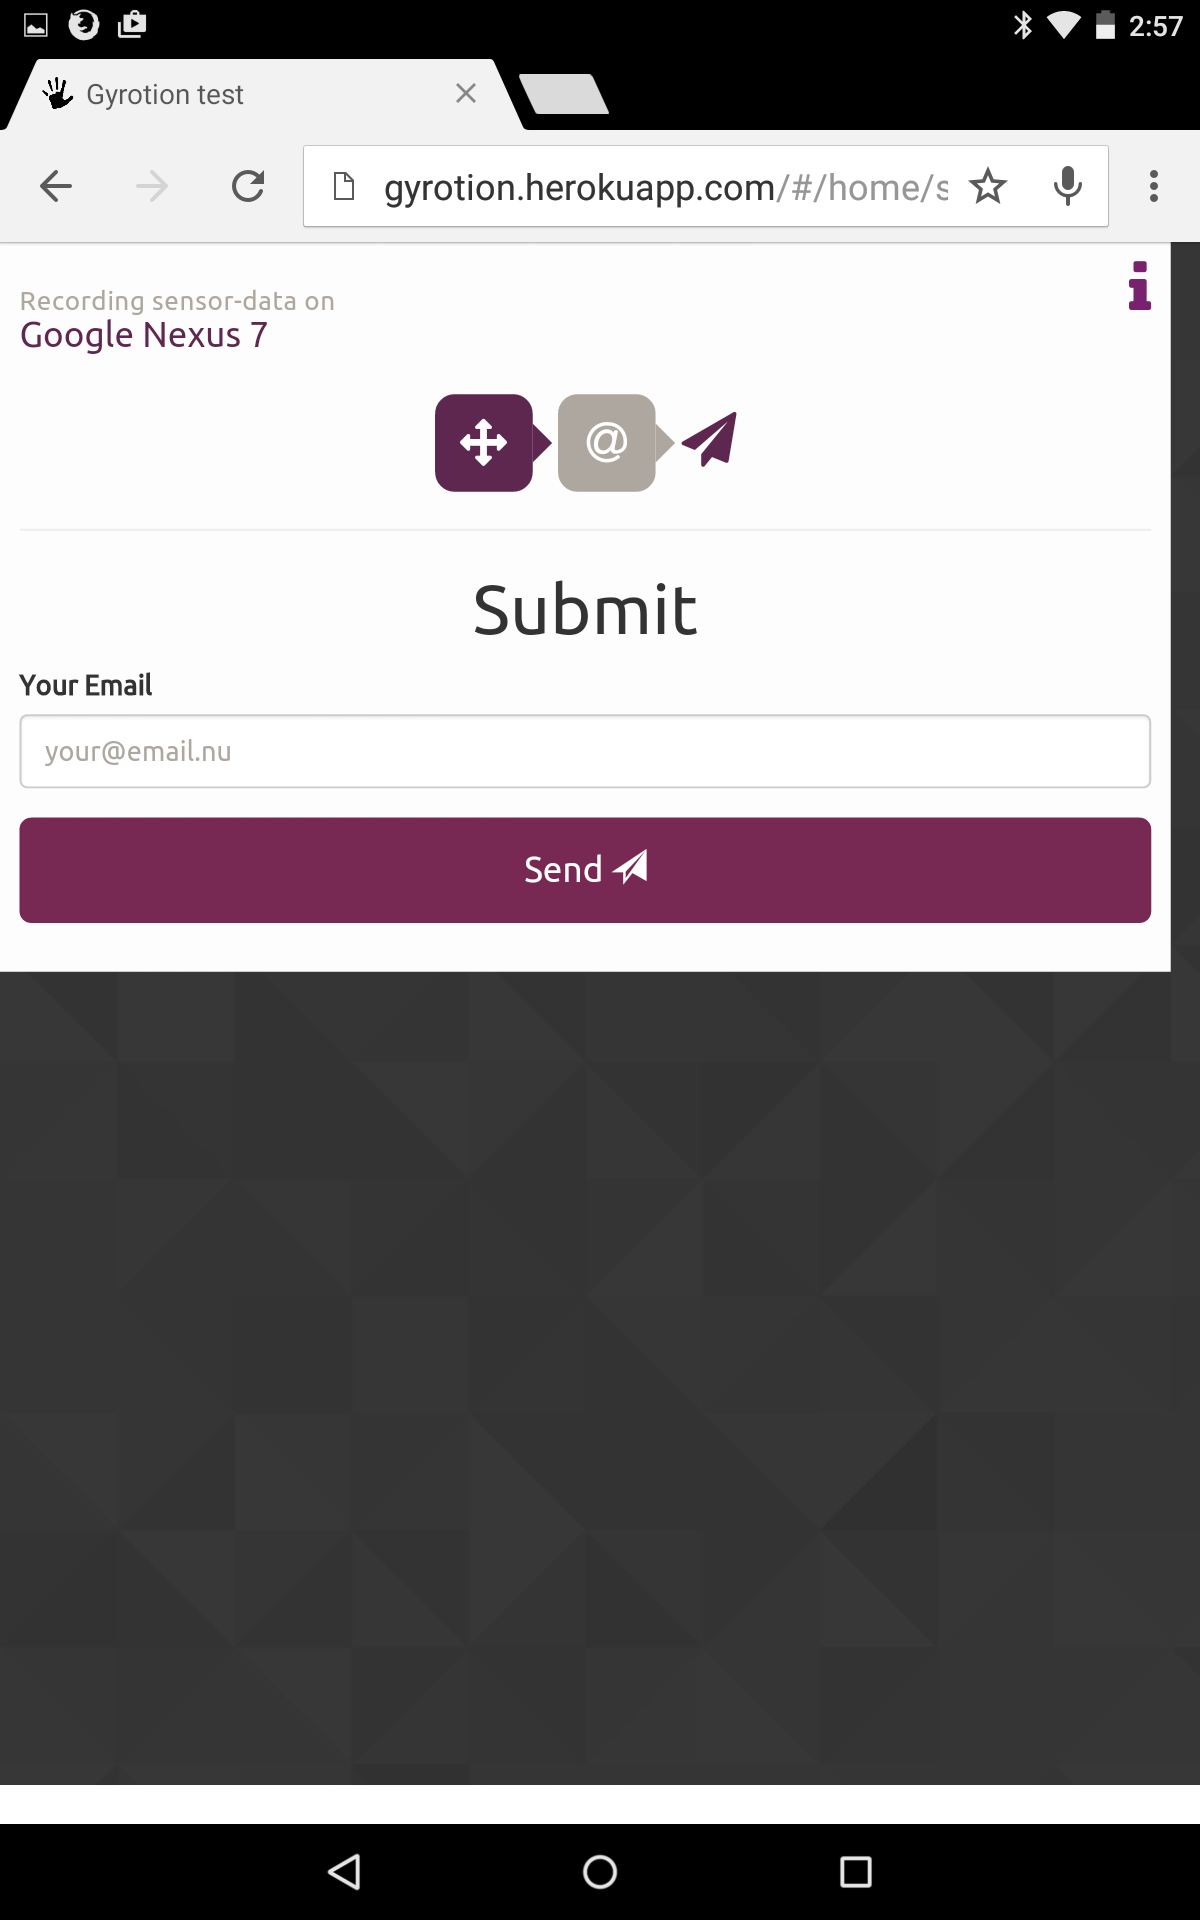
\includegraphics[scale=0.1]{img/Nexus-submit}
  \end{minipage}
  \caption{Screen shot from the page that  made recordings of accelerometer and gyroscope sensors in the first test}
  \label{fig:gyrotion}
\end{figure}

\subsection{Accelerometer \& Gyroscope-test II}

From the last test some changes were made to improve the test result:
\begin{itemize}
  \item Adding time-stamp to every recording sample to know exactly recording frequency
  \item Time based recording on 30 seconds instead of taking 1000 samples as in test I
  \item It's also sampling at a lower rate of at least 10 ms instead of as fast as it could before to reduce the effect of which other processes are in use on the device.
  % Ta bort ngn av pubkterna nedan?
  \item Make 2 recordings with the difference of a 180 degree rotation alpha wise (see \figureref{fig:device-axes}) for better bias estimation \cite{acc:kionixerr}.
  \item Added vibration in the recording to remove environmental noise which is one of the largest noise sources ~\cite[p.8]{acc:kionixerr} 
  \item An additional recording with the device placed in hand to make 
\end{itemize}

\section{Camera}\label{sec:test:camera}
For the test of the camera sensor the PRNU value is calculated as an approximation of the algorithm described in section ~\ref{sec:char:camera} and also used by \cite{sensor:camera:DCIdent}. That is the average of multiple image used and substantially an approximation of \textit{f}. The first step is to remove the image-content which leaves the noise, which is done using a denoising filter. For the test the MATLAB \texttt{medfilt2} is used, which is an 2-D median filtering that outputs the median value of each pixel by its 3-by-3 neighbors. 
\begin{figure}[H]
  \centering
  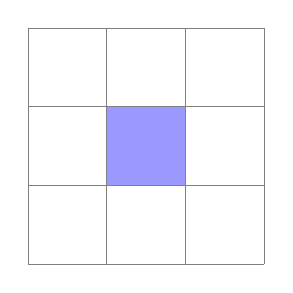
\begin{tikzpicture}[scale=1]
	\draw[step=1cm,gray,very thin] (0,0) grid (3,3);
	\fill[blue!40!white] (1,1) rectangle (2,2);
\end{tikzpicture}
  \caption{\label{fig:medfilt2} the MATLAB \texttt{medfilt2} outputs the median of each pixel by it's 3-by-3 neighbors}
\end{figure}
From the \texttt{medfilt2} we gain a picture without noise which is then subtracted from the original to get the noise. This technique works best if there are no features on the image such auto-fix, black and white etc. The more images used for the average value the better noise is, thus the amount random noise is less and the fixed noise is more. \cite{sensor:camera:DCIdent} recommend a minimum of 50 images. This is then seen as the reference pattern used for correlating the noise from another image. This correlation is calculated like:
$$
corr(\boldsymbol{n},\boldsymbol{r}) = 
\frac{(\boldsymbol{n} - \bar{\boldsymbol{n}})(\boldsymbol{r} - \bar{\boldsymbol{r}})}
{\|\boldsymbol{n} - \bar{\boldsymbol{n}}\| \|\boldsymbol{r} - \bar{\boldsymbol{r}}\|}
$$
A threshold for acceptance on correlation is found by experimental on images taken with or without the camera. Then there is a balance between FAR and FRR. 

\section{Camera test I}
Since the purpose of this thesis compared to earlier work REFERENSER!! has the purpose of authentication and not forensics, is convenience for the collecting and measurability a factor to take in account. That is why the fist experiment is asked the users to record a 5 seconds video-clip with the device camera facing down on a flat object, like a table. Instead of making the user take 50 image or more which takes a lot of more time. This also makes it easier to get better noise since the same scene is used every time. \\
The video is then shuttled into images (100-200 from a 5 seconds video depending on fps on recording camera) that is used for calculating the PRNU. The MATLAB code for this is:\\
\rule{\textwidth}{0.5pt}
  \lstinputlisting{code/video2prnu1.m}
\rule{\textwidth}{0.5pt}

To compare an image between all collected PRNU the same calculation to get the noise is done. Then the noise from the reference image is compared to all collected PRNU and correlation is calculated like the formula above in MATLAB:\\
\rule{\textwidth}{0.5pt}
  \lstinputlisting{code/corrCamTest1.m}
\rule{\textwidth}{0.5pt}

\section{Camera test II}
Since the earlier test leaved out some of the PRNU noise when recorded a video instead of taking a picture the new test consist of 10 images from every device. The recommendation from \cite{sensor:camera:DCIdent} to use at least 50 images is here compensated by again using black images (picture taking with device camera facing down). Since the scene is always the same the noise removal will be better in fewer images. The same code is used as above with the different that the video to image step is removed. The sizes of the images in this case is better since the camera on the mobile devices by default uses higher resolution when taking a picture then when recording. 